% Options for packages loaded elsewhere
\PassOptionsToPackage{unicode}{hyperref}
\PassOptionsToPackage{hyphens}{url}
%
\documentclass[
]{article}
\usepackage{amsmath,amssymb}
\usepackage{lmodern}
\usepackage{iftex}
\ifPDFTeX
  \usepackage[T1]{fontenc}
  \usepackage[utf8]{inputenc}
  \usepackage{textcomp} % provide euro and other symbols
\else % if luatex or xetex
  \usepackage{unicode-math}
  \defaultfontfeatures{Scale=MatchLowercase}
  \defaultfontfeatures[\rmfamily]{Ligatures=TeX,Scale=1}
\fi
% Use upquote if available, for straight quotes in verbatim environments
\IfFileExists{upquote.sty}{\usepackage{upquote}}{}
\IfFileExists{microtype.sty}{% use microtype if available
  \usepackage[]{microtype}
  \UseMicrotypeSet[protrusion]{basicmath} % disable protrusion for tt fonts
}{}
\makeatletter
\@ifundefined{KOMAClassName}{% if non-KOMA class
  \IfFileExists{parskip.sty}{%
    \usepackage{parskip}
  }{% else
    \setlength{\parindent}{0pt}
    \setlength{\parskip}{6pt plus 2pt minus 1pt}}
}{% if KOMA class
  \KOMAoptions{parskip=half}}
\makeatother
\usepackage{xcolor}
\usepackage[margin=1in]{geometry}
\usepackage{color}
\usepackage{fancyvrb}
\newcommand{\VerbBar}{|}
\newcommand{\VERB}{\Verb[commandchars=\\\{\}]}
\DefineVerbatimEnvironment{Highlighting}{Verbatim}{commandchars=\\\{\}}
% Add ',fontsize=\small' for more characters per line
\usepackage{framed}
\definecolor{shadecolor}{RGB}{248,248,248}
\newenvironment{Shaded}{\begin{snugshade}}{\end{snugshade}}
\newcommand{\AlertTok}[1]{\textcolor[rgb]{0.94,0.16,0.16}{#1}}
\newcommand{\AnnotationTok}[1]{\textcolor[rgb]{0.56,0.35,0.01}{\textbf{\textit{#1}}}}
\newcommand{\AttributeTok}[1]{\textcolor[rgb]{0.77,0.63,0.00}{#1}}
\newcommand{\BaseNTok}[1]{\textcolor[rgb]{0.00,0.00,0.81}{#1}}
\newcommand{\BuiltInTok}[1]{#1}
\newcommand{\CharTok}[1]{\textcolor[rgb]{0.31,0.60,0.02}{#1}}
\newcommand{\CommentTok}[1]{\textcolor[rgb]{0.56,0.35,0.01}{\textit{#1}}}
\newcommand{\CommentVarTok}[1]{\textcolor[rgb]{0.56,0.35,0.01}{\textbf{\textit{#1}}}}
\newcommand{\ConstantTok}[1]{\textcolor[rgb]{0.00,0.00,0.00}{#1}}
\newcommand{\ControlFlowTok}[1]{\textcolor[rgb]{0.13,0.29,0.53}{\textbf{#1}}}
\newcommand{\DataTypeTok}[1]{\textcolor[rgb]{0.13,0.29,0.53}{#1}}
\newcommand{\DecValTok}[1]{\textcolor[rgb]{0.00,0.00,0.81}{#1}}
\newcommand{\DocumentationTok}[1]{\textcolor[rgb]{0.56,0.35,0.01}{\textbf{\textit{#1}}}}
\newcommand{\ErrorTok}[1]{\textcolor[rgb]{0.64,0.00,0.00}{\textbf{#1}}}
\newcommand{\ExtensionTok}[1]{#1}
\newcommand{\FloatTok}[1]{\textcolor[rgb]{0.00,0.00,0.81}{#1}}
\newcommand{\FunctionTok}[1]{\textcolor[rgb]{0.00,0.00,0.00}{#1}}
\newcommand{\ImportTok}[1]{#1}
\newcommand{\InformationTok}[1]{\textcolor[rgb]{0.56,0.35,0.01}{\textbf{\textit{#1}}}}
\newcommand{\KeywordTok}[1]{\textcolor[rgb]{0.13,0.29,0.53}{\textbf{#1}}}
\newcommand{\NormalTok}[1]{#1}
\newcommand{\OperatorTok}[1]{\textcolor[rgb]{0.81,0.36,0.00}{\textbf{#1}}}
\newcommand{\OtherTok}[1]{\textcolor[rgb]{0.56,0.35,0.01}{#1}}
\newcommand{\PreprocessorTok}[1]{\textcolor[rgb]{0.56,0.35,0.01}{\textit{#1}}}
\newcommand{\RegionMarkerTok}[1]{#1}
\newcommand{\SpecialCharTok}[1]{\textcolor[rgb]{0.00,0.00,0.00}{#1}}
\newcommand{\SpecialStringTok}[1]{\textcolor[rgb]{0.31,0.60,0.02}{#1}}
\newcommand{\StringTok}[1]{\textcolor[rgb]{0.31,0.60,0.02}{#1}}
\newcommand{\VariableTok}[1]{\textcolor[rgb]{0.00,0.00,0.00}{#1}}
\newcommand{\VerbatimStringTok}[1]{\textcolor[rgb]{0.31,0.60,0.02}{#1}}
\newcommand{\WarningTok}[1]{\textcolor[rgb]{0.56,0.35,0.01}{\textbf{\textit{#1}}}}
\usepackage{graphicx}
\makeatletter
\def\maxwidth{\ifdim\Gin@nat@width>\linewidth\linewidth\else\Gin@nat@width\fi}
\def\maxheight{\ifdim\Gin@nat@height>\textheight\textheight\else\Gin@nat@height\fi}
\makeatother
% Scale images if necessary, so that they will not overflow the page
% margins by default, and it is still possible to overwrite the defaults
% using explicit options in \includegraphics[width, height, ...]{}
\setkeys{Gin}{width=\maxwidth,height=\maxheight,keepaspectratio}
% Set default figure placement to htbp
\makeatletter
\def\fps@figure{htbp}
\makeatother
\setlength{\emergencystretch}{3em} % prevent overfull lines
\providecommand{\tightlist}{%
  \setlength{\itemsep}{0pt}\setlength{\parskip}{0pt}}
\setcounter{secnumdepth}{-\maxdimen} % remove section numbering
\ifLuaTeX
  \usepackage{selnolig}  % disable illegal ligatures
\fi
\IfFileExists{bookmark.sty}{\usepackage{bookmark}}{\usepackage{hyperref}}
\IfFileExists{xurl.sty}{\usepackage{xurl}}{} % add URL line breaks if available
\urlstyle{same} % disable monospaced font for URLs
\hypersetup{
  pdftitle={PSTAT 131/231 Homework 6},
  pdfauthor={William Long},
  hidelinks,
  pdfcreator={LaTeX via pandoc}}

\title{PSTAT 131/231 Homework 6}
\author{William Long}
\date{}

\begin{document}
\maketitle

{
\setcounter{tocdepth}{2}
\tableofcontents
}
\hypertarget{tree-based-models}{%
\subsection{Tree-Based Models}\label{tree-based-models}}

For this assignment, we will continue working with the file
\texttt{"pokemon.csv"}, found in \texttt{/data}. The file is from
Kaggle: \url{https://www.kaggle.com/abcsds/pokemon}.

The \href{https://www.pokemon.com/us/}{Pokémon} franchise encompasses
video games, TV shows, movies, books, and a card game. This data set was
drawn from the video game series and contains statistics about 721
Pokémon, or ``pocket monsters.'' In Pokémon games, the user plays as a
trainer who collects, trades, and battles Pokémon to (a) collect all the
Pokémon and (b) become the champion Pokémon trainer.

Each Pokémon has a
\href{https://bulbapedia.bulbagarden.net/wiki/Type}{primary type} (some
even have secondary types). Based on their type, a Pokémon is strong
against some types, and vulnerable to others. (Think rock, paper,
scissors.) A Fire-type Pokémon, for example, is vulnerable to Water-type
Pokémon, but strong against Grass-type.

\begin{figure}
\centering
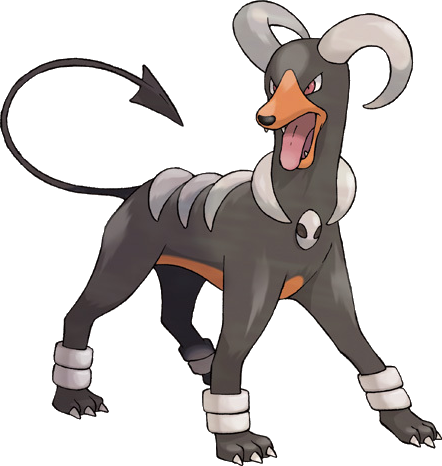
\includegraphics[width=2.08333in,height=\textheight]{images/houndoom.jpg}
\caption{Fig 1. Houndoom, a Dark/Fire-type canine Pokémon from
Generation II.}
\end{figure}

The goal of this assignment is to build a statistical learning model
that can predict the \textbf{primary type} of a Pokémon based on its
generation, legendary status, and six battle statistics.

\textbf{Note: Fitting ensemble tree-based models can take a little while
to run. Consider running your models outside of the .Rmd, storing the
results, and loading them in your .Rmd to minimize time to knit.}

\hypertarget{exercise-1}{%
\subsubsection{Exercise 1}\label{exercise-1}}

Read in the data and set things up as in Homework 5:

\begin{itemize}
\tightlist
\item
  Use \texttt{clean\_names()}
\item
  Filter out the rarer Pokémon types
\item
  Convert \texttt{type\_1} and \texttt{legendary} to factors
\end{itemize}

Do an initial split of the data; you can choose the percentage for
splitting. Stratify on the outcome variable.

Fold the training set using \emph{v}-fold cross-validation, with
\texttt{v\ =\ 5}. Stratify on the outcome variable.

Set up a recipe to predict \texttt{type\_1} with \texttt{legendary},
\texttt{generation}, \texttt{sp\_atk}, \texttt{attack}, \texttt{speed},
\texttt{defense}, \texttt{hp}, and \texttt{sp\_def}:

\begin{itemize}
\tightlist
\item
  Dummy-code \texttt{legendary} and \texttt{generation};
\item
  Center and scale all predictors.
\end{itemize}

\begin{Shaded}
\begin{Highlighting}[]
\CommentTok{\#Reading in data}
\CommentTok{\#setwd("C:/Users/William/Desktop/PSTAT{-}131{-}HW6")}
\NormalTok{pokemon }\OtherTok{\textless{}{-}} \FunctionTok{read.csv}\NormalTok{(}\StringTok{"data/Pokemon.csv"}\NormalTok{)}

\NormalTok{pokemon\_clean }\OtherTok{\textless{}{-}} \FunctionTok{clean\_names}\NormalTok{(pokemon)}

\CommentTok{\#Filtering out rarer types}
\NormalTok{pokemon\_filter }\OtherTok{\textless{}{-}}\NormalTok{ pokemon\_clean }\SpecialCharTok{\%\textgreater{}\%}
  \FunctionTok{filter}\NormalTok{(type\_1 }\SpecialCharTok{==} \StringTok{"Bug"} \SpecialCharTok{|}\NormalTok{ type\_1 }\SpecialCharTok{==} \StringTok{"Fire"} \SpecialCharTok{|}\NormalTok{ type\_1 }\SpecialCharTok{==} \StringTok{"Grass"} \SpecialCharTok{|}\NormalTok{ type\_1 }\SpecialCharTok{==} \StringTok{"Normal"} \SpecialCharTok{|}
\NormalTok{           type\_1 }\SpecialCharTok{==} \StringTok{"Water"} \SpecialCharTok{|}\NormalTok{ type\_1 }\SpecialCharTok{==} \StringTok{"Psychic"}\NormalTok{)}

\CommentTok{\#Converting type, legendary, and generation to factor variables}
\NormalTok{pokemon\_filter}\SpecialCharTok{$}\NormalTok{type\_1 }\OtherTok{\textless{}{-}} \FunctionTok{factor}\NormalTok{(pokemon\_filter}\SpecialCharTok{$}\NormalTok{type\_1)}
\NormalTok{pokemon\_filter}\SpecialCharTok{$}\NormalTok{legendary }\OtherTok{\textless{}{-}} \FunctionTok{factor}\NormalTok{(pokemon\_filter}\SpecialCharTok{$}\NormalTok{legendary)}
\NormalTok{pokemon\_filter}\SpecialCharTok{$}\NormalTok{generation }\OtherTok{\textless{}{-}} \FunctionTok{factor}\NormalTok{(pokemon\_filter}\SpecialCharTok{$}\NormalTok{generation)}

\CommentTok{\#Splitting the data}
\FunctionTok{set.seed}\NormalTok{(}\DecValTok{2012}\NormalTok{)}
\NormalTok{pokemon\_split }\OtherTok{\textless{}{-}} \FunctionTok{initial\_split}\NormalTok{(pokemon\_filter, }\AttributeTok{prop =} \FloatTok{0.7}\NormalTok{, }\AttributeTok{strata =}\NormalTok{ type\_1)}
\NormalTok{pokemon\_train }\OtherTok{\textless{}{-}} \FunctionTok{training}\NormalTok{(pokemon\_split)}
\NormalTok{pokemon\_test }\OtherTok{\textless{}{-}} \FunctionTok{testing}\NormalTok{(pokemon\_split)}

\CommentTok{\#Creating folds on the training data}
\NormalTok{pokemon\_folds }\OtherTok{\textless{}{-}} \FunctionTok{vfold\_cv}\NormalTok{(pokemon\_train, }\AttributeTok{v=}\DecValTok{5}\NormalTok{, }\AttributeTok{strata =}\NormalTok{ type\_1)}

\CommentTok{\#Recipe}
\NormalTok{pokemon\_recipe }\OtherTok{\textless{}{-}} \FunctionTok{recipe}\NormalTok{(type\_1 }\SpecialCharTok{\textasciitilde{}}\NormalTok{ legendary }\SpecialCharTok{+}\NormalTok{ generation }\SpecialCharTok{+}\NormalTok{ sp\_atk }\SpecialCharTok{+}\NormalTok{ attack }\SpecialCharTok{+}\NormalTok{ speed }\SpecialCharTok{+}\NormalTok{ defense }\SpecialCharTok{+}\NormalTok{ hp }\SpecialCharTok{+}\NormalTok{ sp\_def, }\AttributeTok{data =}\NormalTok{ pokemon\_train) }\SpecialCharTok{\%\textgreater{}\%}
  \FunctionTok{step\_dummy}\NormalTok{(legendary) }\SpecialCharTok{\%\textgreater{}\%}    \CommentTok{\#Dummy{-}coding categorical predictors}
  \FunctionTok{step\_dummy}\NormalTok{(generation) }\SpecialCharTok{\%\textgreater{}\%}
  \FunctionTok{step\_normalize}\NormalTok{(}\FunctionTok{all\_predictors}\NormalTok{()) }\CommentTok{\#Centering and scaling}
\end{Highlighting}
\end{Shaded}

\hypertarget{exercise-2}{%
\subsubsection{Exercise 2}\label{exercise-2}}

Create a correlation matrix of the training set, using the
\texttt{corrplot} package. \emph{Note: You can choose how to handle the
continuous variables for this plot; justify your decision(s).}

What relationships, if any, do you notice? Do these relationships make
sense to you?

\begin{Shaded}
\begin{Highlighting}[]
\CommentTok{\#Transform non{-}continuous variables to continuous if possible}
\CommentTok{\#because correlation is best done between numeric and contininous variables}
\NormalTok{pokemon\_matrix\_df }\OtherTok{\textless{}{-}} \FunctionTok{select}\NormalTok{(pokemon\_train, }\FunctionTok{c}\NormalTok{(}\StringTok{\textquotesingle{}type\_1\textquotesingle{}}\NormalTok{,}\StringTok{\textquotesingle{}legendary\textquotesingle{}}\NormalTok{,}\StringTok{\textquotesingle{}generation\textquotesingle{}}\NormalTok{,}\StringTok{\textquotesingle{}sp\_atk\textquotesingle{}}\NormalTok{,}\StringTok{\textquotesingle{}attack\textquotesingle{}}\NormalTok{,}\StringTok{\textquotesingle{}speed\textquotesingle{}}\NormalTok{,}\StringTok{\textquotesingle{}defense\textquotesingle{}}\NormalTok{,}\StringTok{\textquotesingle{}hp\textquotesingle{}}\NormalTok{,}\StringTok{\textquotesingle{}sp\_def\textquotesingle{}}\NormalTok{)) }\SpecialCharTok{\%\textgreater{}\%}
  \FunctionTok{mutate\_if}\NormalTok{(is.character, as.factor) }\SpecialCharTok{\%\textgreater{}\%}
  \FunctionTok{mutate\_if}\NormalTok{(is.factor, as.numeric)}

\NormalTok{pokemon\_corr\_matrix }\OtherTok{\textless{}{-}} \FunctionTok{cor}\NormalTok{(pokemon\_matrix\_df)}

\FunctionTok{corrplot}\NormalTok{(pokemon\_corr\_matrix, }\AttributeTok{method =} \StringTok{"number"}\NormalTok{)}
\end{Highlighting}
\end{Shaded}

\includegraphics{homework-6_files/figure-latex/corr-1.pdf} A: Defense
and special defense seem to have a decent amount of correlation. This
makes sense because most Pokemon that are on the bulkier side usually
don't have a glaring weakness against either physical or special
attackers. Glass cannon Pokemon also tend to be low on both of those
stats. Attack and speed also seem to have a relationship, likely because
offensive Pokemon tend to have high numbers in both of those stats.
Legendary Pokemon are also correlated more with special attack than
other stat. This makes sense, because these Pokemon tend to possess
unique and/or flashy moves which are more likely to be special attacking
moves instead of physical moves. Each attack stat(special attack and
attack) and their corresponding defense stat(special defense and
defense) also seem to have a relationship, which I think makes sense
intuitively. {[}Maybe edit this?{]}

\hypertarget{exercise-3}{%
\subsubsection{Exercise 3}\label{exercise-3}}

First, set up a decision tree model and workflow. Tune the
\texttt{cost\_complexity} hyperparameter. Use the same levels we used in
Lab 7 -- that is, \texttt{range\ =\ c(-3,\ -1)}. Specify that the metric
we want to optimize is \texttt{roc\_auc}.

Print an \texttt{autoplot()} of the results. What do you observe? Does a
single decision tree perform better with a smaller or larger complexity
penalty?

\begin{Shaded}
\begin{Highlighting}[]
\CommentTok{\#Classification decision tree}
\NormalTok{class\_tree\_spec }\OtherTok{\textless{}{-}} \FunctionTok{decision\_tree}\NormalTok{() }\SpecialCharTok{\%\textgreater{}\%}
  \FunctionTok{set\_engine}\NormalTok{(}\StringTok{"rpart"}\NormalTok{) }\SpecialCharTok{\%\textgreater{}\%}
  \FunctionTok{set\_mode}\NormalTok{(}\StringTok{"classification"}\NormalTok{)}

\CommentTok{\#Workflow with tuning parameter}
\NormalTok{class\_tree\_wf }\OtherTok{\textless{}{-}} \FunctionTok{workflow}\NormalTok{() }\SpecialCharTok{\%\textgreater{}\%}
  \FunctionTok{add\_model}\NormalTok{(class\_tree\_spec }\SpecialCharTok{\%\textgreater{}\%} \FunctionTok{set\_args}\NormalTok{(}\AttributeTok{cost\_complexity =} \FunctionTok{tune}\NormalTok{())) }\SpecialCharTok{\%\textgreater{}\%}
  \FunctionTok{add\_recipe}\NormalTok{(pokemon\_recipe)}

\CommentTok{\#cost\_complexity hyperparameter}
\NormalTok{param\_grid }\OtherTok{\textless{}{-}} \FunctionTok{grid\_regular}\NormalTok{(}\FunctionTok{cost\_complexity}\NormalTok{(}\AttributeTok{range =} \FunctionTok{c}\NormalTok{(}\SpecialCharTok{{-}}\DecValTok{3}\NormalTok{, }\SpecialCharTok{{-}}\DecValTok{1}\NormalTok{)), }\AttributeTok{levels =} \DecValTok{10}\NormalTok{)}

\NormalTok{tune\_res }\OtherTok{\textless{}{-}} \FunctionTok{tune\_grid}\NormalTok{(}
\NormalTok{  class\_tree\_wf, }
  \AttributeTok{resamples =}\NormalTok{ pokemon\_folds, }
  \AttributeTok{grid =}\NormalTok{ param\_grid, }
  \AttributeTok{metrics =} \FunctionTok{metric\_set}\NormalTok{(roc\_auc)}
\NormalTok{)}

\FunctionTok{autoplot}\NormalTok{(tune\_res)}
\end{Highlighting}
\end{Shaded}

\includegraphics{homework-6_files/figure-latex/tree-1.pdf}

A: As seen in the graph, the ROC\_AUC starts off relatively high with
low complexity penalty level, then peaks between 0.01 and 0.1, and then
falls off rather steeply. Thus, a single decision tree appears to
perform better with a smaller complexity penalty because the ROC\_AUC
will quickly plummet after increasing the complexity penalty after a
certain point.

\hypertarget{exercise-4}{%
\subsubsection{Exercise 4}\label{exercise-4}}

What is the \texttt{roc\_auc} of your best-performing pruned decision
tree on the folds? \emph{Hint: Use \texttt{collect\_metrics()} and
\texttt{arrange()}.}

\begin{Shaded}
\begin{Highlighting}[]
\NormalTok{best\_complexity }\OtherTok{\textless{}{-}} \FunctionTok{select\_best}\NormalTok{(tune\_res, }\AttributeTok{metric =} \StringTok{"roc\_auc"}\NormalTok{)}

\FunctionTok{collect\_metrics}\NormalTok{(tune\_res) }\SpecialCharTok{\%\textgreater{}\%} \FunctionTok{arrange}\NormalTok{(}\FunctionTok{desc}\NormalTok{(mean)) }\SpecialCharTok{\%\textgreater{}\%} \FunctionTok{head}\NormalTok{(}\DecValTok{1}\NormalTok{)}
\end{Highlighting}
\end{Shaded}

\begin{verbatim}
## # A tibble: 1 x 7
##   cost_complexity .metric .estimator  mean     n std_err .config              
##             <dbl> <chr>   <chr>      <dbl> <int>   <dbl> <chr>                
## 1          0.0359 roc_auc hand_till  0.640     5  0.0181 Preprocessor1_Model08
\end{verbatim}

A: The ROC\_AUC of my best-performing pruned decision tree is 0.6401222.

\hypertarget{exercise-5}{%
\subsubsection{Exercise 5}\label{exercise-5}}

Using \texttt{rpart.plot}, fit and visualize your best-performing pruned
decision tree with the \emph{training} set.

\begin{Shaded}
\begin{Highlighting}[]
\NormalTok{class\_tree\_final }\OtherTok{\textless{}{-}} \FunctionTok{finalize\_workflow}\NormalTok{(class\_tree\_wf, best\_complexity)}

\NormalTok{class\_tree\_final\_fit }\OtherTok{\textless{}{-}} \FunctionTok{fit}\NormalTok{(class\_tree\_final, }\AttributeTok{data =}\NormalTok{ pokemon\_train)}

\NormalTok{class\_tree\_final\_fit }\SpecialCharTok{\%\textgreater{}\%}
  \FunctionTok{extract\_fit\_engine}\NormalTok{() }\SpecialCharTok{\%\textgreater{}\%}
  \FunctionTok{rpart.plot}\NormalTok{()}
\end{Highlighting}
\end{Shaded}

\includegraphics{homework-6_files/figure-latex/bestFit-1.pdf}

\hypertarget{exercise-5-1}{%
\subsubsection{Exercise 5}\label{exercise-5-1}}

Now set up a random forest model and workflow. Use the \texttt{ranger}
engine and set \texttt{importance\ =\ "impurity"}. Tune \texttt{mtry},
\texttt{trees}, and \texttt{min\_n}. Using the documentation for
\texttt{rand\_forest()}, explain in your own words what each of these
hyperparameters represent.

Create a regular grid with 8 levels each. You can choose plausible
ranges for each hyperparameter. Note that \texttt{mtry} should not be
smaller than 1 or larger than 8. \textbf{Explain why not. What type of
model would \texttt{mtry\ =\ 8} represent?}

\begin{Shaded}
\begin{Highlighting}[]
\NormalTok{rf\_spec }\OtherTok{\textless{}{-}} \FunctionTok{rand\_forest}\NormalTok{() }\SpecialCharTok{\%\textgreater{}\%}
  \FunctionTok{set\_engine}\NormalTok{(}\StringTok{"ranger"}\NormalTok{, }\AttributeTok{importance =} \StringTok{"impurity"}\NormalTok{) }\SpecialCharTok{\%\textgreater{}\%}
  \FunctionTok{set\_mode}\NormalTok{(}\StringTok{"classification"}\NormalTok{)}

\CommentTok{\#Tuning parameters}
\NormalTok{rf\_wf }\OtherTok{\textless{}{-}} \FunctionTok{workflow}\NormalTok{() }\SpecialCharTok{\%\textgreater{}\%}
  \FunctionTok{add\_model}\NormalTok{(rf\_spec }\SpecialCharTok{\%\textgreater{}\%} \FunctionTok{set\_args}\NormalTok{(}\AttributeTok{mtry =} \FunctionTok{tune}\NormalTok{(), }\AttributeTok{trees =} \FunctionTok{tune}\NormalTok{(), }\AttributeTok{min\_n =} \FunctionTok{tune}\NormalTok{())) }\SpecialCharTok{\%\textgreater{}\%}
  \FunctionTok{add\_recipe}\NormalTok{(pokemon\_recipe)}

\NormalTok{rf\_param\_grid }\OtherTok{\textless{}{-}} \FunctionTok{grid\_regular}\NormalTok{(}\FunctionTok{mtry}\NormalTok{(}\AttributeTok{range=}\FunctionTok{c}\NormalTok{(}\DecValTok{1}\NormalTok{,}\DecValTok{8}\NormalTok{)), }\FunctionTok{trees}\NormalTok{(}\AttributeTok{range=}\FunctionTok{c}\NormalTok{(}\DecValTok{64}\NormalTok{,}\DecValTok{128}\NormalTok{)), }\FunctionTok{min\_n}\NormalTok{(}\AttributeTok{range =} \FunctionTok{c}\NormalTok{(}\DecValTok{10}\NormalTok{, }\DecValTok{100}\NormalTok{)), }\AttributeTok{levels =} \DecValTok{8}\NormalTok{)}
\end{Highlighting}
\end{Shaded}

A: ``mtry'' represents how many predictors that are randomly sampled at
each tree split.

``trees'' is the total number of trees made in the model.

``min\_n'' represents the minimum number of data points needed in a node
to perform another split.

Since ``mtry'' is the number of predictors that will be randomly
sampled, it cannot be less than 1 because then there is no data to
predict from and it cannot be greater than 8 because we don't have more
than 8 predictors in our recipe. A model with ``mtry'' = 8 would
represent a bagging model.

\hypertarget{exercise-6}{%
\subsubsection{Exercise 6}\label{exercise-6}}

Specify \texttt{roc\_auc} as a metric. Tune the model and print an
\texttt{autoplot()} of the results. What do you observe? What values of
the hyperparameters seem to yield the best performance?

\begin{Shaded}
\begin{Highlighting}[]
\NormalTok{tune\_res\_rf }\OtherTok{\textless{}{-}} \FunctionTok{tune\_grid}\NormalTok{(}
\NormalTok{  rf\_wf, }
  \AttributeTok{resamples =}\NormalTok{ pokemon\_folds, }
  \AttributeTok{grid =}\NormalTok{ rf\_param\_grid, }
  \AttributeTok{metrics =} \FunctionTok{metric\_set}\NormalTok{(roc\_auc)}
\NormalTok{)}

\FunctionTok{save}\NormalTok{(tune\_res\_rf, }\AttributeTok{file =} \StringTok{"tune\_res\_rf.rda"}\NormalTok{)}
\end{Highlighting}
\end{Shaded}

\begin{Shaded}
\begin{Highlighting}[]
\FunctionTok{load}\NormalTok{(}\AttributeTok{file =} \StringTok{"tune\_res\_rf.rda"}\NormalTok{ )}
\FunctionTok{autoplot}\NormalTok{(tune\_res\_rf)}
\end{Highlighting}
\end{Shaded}

\includegraphics{homework-6_files/figure-latex/unnamed-chunk-1-1.pdf}

A: 3 randomly selected predictors, a minimal node size of 22, and 128
trees seems to yield the best performance according to the graphs.

\hypertarget{exercise-7}{%
\subsubsection{Exercise 7}\label{exercise-7}}

What is the \texttt{roc\_auc} of your best-performing random forest
model on the folds? \emph{Hint: Use \texttt{collect\_metrics()} and
\texttt{arrange()}.}

\begin{Shaded}
\begin{Highlighting}[]
\NormalTok{best\_params\_rf }\OtherTok{\textless{}{-}} \FunctionTok{select\_best}\NormalTok{(tune\_res\_rf)}

\FunctionTok{collect\_metrics}\NormalTok{(tune\_res\_rf) }\SpecialCharTok{\%\textgreater{}\%} \FunctionTok{arrange}\NormalTok{(}\FunctionTok{desc}\NormalTok{(mean)) }\SpecialCharTok{\%\textgreater{}\%} \FunctionTok{head}\NormalTok{(}\DecValTok{1}\NormalTok{)}
\end{Highlighting}
\end{Shaded}

\begin{verbatim}
## # A tibble: 1 x 9
##    mtry trees min_n .metric .estimator  mean     n std_err .config              
##   <int> <int> <int> <chr>   <chr>      <dbl> <int>   <dbl> <chr>                
## 1     3   128    22 roc_auc hand_till  0.728     5  0.0165 Preprocessor1_Model1~
\end{verbatim}

A: The ROC\_AUC of my best performing random forest model was 0.7277884.

\hypertarget{exercise-8}{%
\subsubsection{Exercise 8}\label{exercise-8}}

Create a variable importance plot, using \texttt{vip()}, with your
best-performing random forest model fit on the \emph{training} set.

Which variables were most useful? Which were least useful? Are these
results what you expected, or not?

\begin{Shaded}
\begin{Highlighting}[]
\NormalTok{rf\_final }\OtherTok{\textless{}{-}} \FunctionTok{finalize\_workflow}\NormalTok{(rf\_wf, best\_params\_rf)}
\NormalTok{rf\_final\_fit }\OtherTok{\textless{}{-}} \FunctionTok{fit}\NormalTok{(rf\_final, pokemon\_train)}

\NormalTok{rf\_final\_fit }\SpecialCharTok{\%\textgreater{}\%}
  \FunctionTok{pull\_workflow\_fit}\NormalTok{() }\SpecialCharTok{\%\textgreater{}\%}
  \FunctionTok{vip}\NormalTok{()}
\end{Highlighting}
\end{Shaded}

\includegraphics{homework-6_files/figure-latex/unnamed-chunk-2-1.pdf}

A: Special attack was the most useful. Speed, attack, defense, HP, and
special defense were all about equally important. Generation and
legendary status seemed to be the least useful.

These results are about what I expected. Generation and legendary don't
really indicate a Pokemon's type since each generation releases a ton of
new Pokemon of a wide variety of types and legendaries also vary wildly
in type as well. Pokemon stats ended up being the most useful because
many types fit into traditional archetypes. The only surprising result
for me was that special attack ended up being the most important stat
for predicting primary type.

\hypertarget{exercise-9}{%
\subsubsection{Exercise 9}\label{exercise-9}}

Finally, set up a boosted tree model and workflow. Use the
\texttt{xgboost} engine. Tune \texttt{trees}. Create a regular grid with
10 levels; let \texttt{trees} range from 10 to 2000. Specify
\texttt{roc\_auc} and again print an \texttt{autoplot()} of the results.

\begin{Shaded}
\begin{Highlighting}[]
\NormalTok{boost\_spec }\OtherTok{\textless{}{-}} \FunctionTok{boost\_tree}\NormalTok{() }\SpecialCharTok{\%\textgreater{}\%}
  \FunctionTok{set\_engine}\NormalTok{(}\StringTok{"xgboost"}\NormalTok{) }\SpecialCharTok{\%\textgreater{}\%}
  \FunctionTok{set\_mode}\NormalTok{(}\StringTok{"classification"}\NormalTok{)}

\NormalTok{boost\_wf }\OtherTok{\textless{}{-}} \FunctionTok{workflow}\NormalTok{() }\SpecialCharTok{\%\textgreater{}\%}
  \FunctionTok{add\_model}\NormalTok{(boost\_spec }\SpecialCharTok{\%\textgreater{}\%} \FunctionTok{set\_args}\NormalTok{(}\AttributeTok{trees =} \FunctionTok{tune}\NormalTok{())) }\SpecialCharTok{\%\textgreater{}\%}
  \FunctionTok{add\_recipe}\NormalTok{(pokemon\_recipe)}

\NormalTok{boost\_param\_grid }\OtherTok{\textless{}{-}} \FunctionTok{grid\_regular}\NormalTok{(}\FunctionTok{trees}\NormalTok{(}\AttributeTok{range =} \FunctionTok{c}\NormalTok{(}\DecValTok{10}\NormalTok{, }\DecValTok{2000}\NormalTok{)), }\AttributeTok{levels =} \DecValTok{10}\NormalTok{)}

\NormalTok{tune\_res\_boost }\OtherTok{\textless{}{-}} \FunctionTok{tune\_grid}\NormalTok{(}
\NormalTok{  boost\_wf, }
  \AttributeTok{resamples =}\NormalTok{ pokemon\_folds, }
  \AttributeTok{grid =}\NormalTok{ boost\_param\_grid, }
  \AttributeTok{metrics =} \FunctionTok{metric\_set}\NormalTok{(roc\_auc)}
\NormalTok{)}

\FunctionTok{autoplot}\NormalTok{(tune\_res\_boost)}
\end{Highlighting}
\end{Shaded}

\includegraphics{homework-6_files/figure-latex/boost-1.pdf}

What do you observe?

A: The ROC\_AUC increases steadily as the number of trees increase until
it peaks around 0.71 at approximately 250 trees, then the ROC\_AUC
steadily decreases as the number of trees increases.

What is the \texttt{roc\_auc} of your best-performing boosted tree model
on the folds? \emph{Hint: Use \texttt{collect\_metrics()} and
\texttt{arrange()}.}

\begin{Shaded}
\begin{Highlighting}[]
\FunctionTok{collect\_metrics}\NormalTok{(tune\_res\_boost) }\SpecialCharTok{\%\textgreater{}\%} \FunctionTok{arrange}\NormalTok{(}\FunctionTok{desc}\NormalTok{(mean)) }\SpecialCharTok{\%\textgreater{}\%} \FunctionTok{head}\NormalTok{(}\DecValTok{1}\NormalTok{)}
\end{Highlighting}
\end{Shaded}

\begin{verbatim}
## # A tibble: 1 x 7
##   trees .metric .estimator  mean     n std_err .config              
##   <int> <chr>   <chr>      <dbl> <int>   <dbl> <chr>                
## 1   231 roc_auc hand_till  0.710     5  0.0180 Preprocessor1_Model02
\end{verbatim}

A: The ROC\_AUC of my best-performing boosted tree model is 0.7104561.

\hypertarget{exercise-10}{%
\subsubsection{Exercise 10}\label{exercise-10}}

Display a table of the three ROC AUC values for your best-performing
pruned tree, random forest, and boosted tree models. Which performed
best on the folds? Select the best of the three and use
\texttt{select\_best()}, \texttt{finalize\_workflow()}, and
\texttt{fit()} to fit it to the \emph{testing} set.

Print the AUC value of your best-performing model on the testing set.
Print the ROC curves. Finally, create and visualize a confusion matrix
heat map.

Which classes was your model most accurate at predicting? Which was it
worst at?

\begin{Shaded}
\begin{Highlighting}[]
\NormalTok{pruned\_tree\_metrics }\OtherTok{\textless{}{-}} \FunctionTok{collect\_metrics}\NormalTok{(tune\_res) }\SpecialCharTok{\%\textgreater{}\%} \FunctionTok{arrange}\NormalTok{(}\FunctionTok{desc}\NormalTok{(mean))}
\NormalTok{best\_pruned\_tree }\OtherTok{\textless{}{-}}\NormalTok{ pruned\_tree\_metrics[}\DecValTok{1}\NormalTok{, }\StringTok{\textquotesingle{}mean\textquotesingle{}}\NormalTok{]}

\NormalTok{rf\_metrics }\OtherTok{\textless{}{-}} \FunctionTok{collect\_metrics}\NormalTok{(tune\_res\_rf) }\SpecialCharTok{\%\textgreater{}\%} \FunctionTok{arrange}\NormalTok{(}\FunctionTok{desc}\NormalTok{(mean))}
\NormalTok{best\_rf }\OtherTok{\textless{}{-}}\NormalTok{ rf\_metrics[}\DecValTok{1}\NormalTok{, }\StringTok{\textquotesingle{}mean\textquotesingle{}}\NormalTok{]}

\NormalTok{boost\_metrics }\OtherTok{\textless{}{-}} \FunctionTok{collect\_metrics}\NormalTok{(tune\_res\_boost) }\SpecialCharTok{\%\textgreater{}\%} \FunctionTok{arrange}\NormalTok{(}\FunctionTok{desc}\NormalTok{(mean))}
\NormalTok{best\_boost }\OtherTok{\textless{}{-}}\NormalTok{ boost\_metrics[}\DecValTok{1}\NormalTok{, }\StringTok{\textquotesingle{}mean\textquotesingle{}}\NormalTok{]}

\FunctionTok{bind\_rows}\NormalTok{(best\_pruned\_tree, best\_rf, best\_boost) }\SpecialCharTok{\%\textgreater{}\%} \FunctionTok{mutate}\NormalTok{(}\AttributeTok{model =} \FunctionTok{c}\NormalTok{(}\StringTok{\textquotesingle{}Pruned Tree\textquotesingle{}}\NormalTok{, }\StringTok{\textquotesingle{}Random Forest\textquotesingle{}}\NormalTok{, }\StringTok{\textquotesingle{}Boosted Tree\textquotesingle{}}\NormalTok{))}
\end{Highlighting}
\end{Shaded}

\begin{verbatim}
## # A tibble: 3 x 2
##    mean model        
##   <dbl> <chr>        
## 1 0.640 Pruned Tree  
## 2 0.728 Random Forest
## 3 0.710 Boosted Tree
\end{verbatim}

\begin{Shaded}
\begin{Highlighting}[]
\CommentTok{\#Random forest performed the best}

\CommentTok{\#Fitting best random forest model onto testing data}
\NormalTok{pokemon\_final }\OtherTok{\textless{}{-}} \FunctionTok{finalize\_workflow}\NormalTok{(rf\_wf, best\_params\_rf)}
\NormalTok{pokemon\_final\_fit }\OtherTok{\textless{}{-}} \FunctionTok{fit}\NormalTok{(pokemon\_final, }\AttributeTok{data =}\NormalTok{ pokemon\_test)}
\NormalTok{pokemon\_final\_fit\_test }\OtherTok{\textless{}{-}} \FunctionTok{augment}\NormalTok{(pokemon\_final\_fit, }\AttributeTok{new\_data =}\NormalTok{ pokemon\_test)}

\CommentTok{\#Printing AUC of random forest on testing data}
\FunctionTok{roc\_auc}\NormalTok{(}\AttributeTok{data =}\NormalTok{ pokemon\_final\_fit\_test, }\AttributeTok{truth =}\NormalTok{ type\_1, }\AttributeTok{estimate =} \FunctionTok{c}\NormalTok{(.pred\_Bug, .pred\_Fire, .pred\_Grass, .pred\_Normal, .pred\_Psychic, .pred\_Water)) }\SpecialCharTok{\%\textgreater{}\%} \FunctionTok{print}\NormalTok{()}
\end{Highlighting}
\end{Shaded}

\begin{verbatim}
## # A tibble: 1 x 3
##   .metric .estimator .estimate
##   <chr>   <chr>          <dbl>
## 1 roc_auc hand_till      0.971
\end{verbatim}

\begin{Shaded}
\begin{Highlighting}[]
\CommentTok{\#Plotting ROC curves}
\FunctionTok{augment}\NormalTok{(pokemon\_final\_fit, pokemon\_test) }\SpecialCharTok{\%\textgreater{}\%} \FunctionTok{roc\_curve}\NormalTok{(}\AttributeTok{truth =}\NormalTok{ type\_1, }\AttributeTok{estimate =} \FunctionTok{c}\NormalTok{(.pred\_Bug, .pred\_Fire, .pred\_Grass, .pred\_Normal, .pred\_Water, .pred\_Psychic)) }\SpecialCharTok{\%\textgreater{}\%} \FunctionTok{autoplot}\NormalTok{()}
\end{Highlighting}
\end{Shaded}

\includegraphics{homework-6_files/figure-latex/testing-1.pdf}

\begin{Shaded}
\begin{Highlighting}[]
\FunctionTok{augment}\NormalTok{(pokemon\_final\_fit, }\AttributeTok{new\_data =}\NormalTok{ pokemon\_test) }\SpecialCharTok{\%\textgreater{}\%}
  \FunctionTok{conf\_mat}\NormalTok{(}\AttributeTok{truth =}\NormalTok{ type\_1, }\AttributeTok{estimate =}\NormalTok{ .pred\_class) }\SpecialCharTok{\%\textgreater{}\%} 
  \FunctionTok{autoplot}\NormalTok{(}\AttributeTok{type =} \StringTok{"heatmap"}\NormalTok{)}
\end{Highlighting}
\end{Shaded}

\includegraphics{homework-6_files/figure-latex/testing-2.pdf}

A: My model was most accurate at predicting Normal, Bug, Fire, and Grass
types. It struggled with predicting Psychic and Water types.

\hypertarget{for-231-students}{%
\subsection{For 231 Students}\label{for-231-students}}

\hypertarget{exercise-11}{%
\subsubsection{Exercise 11}\label{exercise-11}}

Using the \texttt{abalone.txt} data from previous assignments, fit and
tune a random forest model to predict \texttt{age}. Use stratified
cross-validation and select ranges for \texttt{mtry}, \texttt{min\_n},
and \texttt{trees}. Present your results. What was the model's RMSE on
your testing set?

\end{document}
